\chapter{Fondamenti}

\section{Intrusion Detection System}


Un intrusione può essere definita come un evento che causa danni ad un sistema informatico ~\cite{SurveyIntrusionDetection2019}.

Gli Intrusion Detection System (IDS) sono delle soluzioni hardware o software che, posti all'interno di una rete o di un sistema, rilevano eventuali intrusioni. 

~\cite{ashoorImportanceIntrusionDetection2010} Le principali funzioni degli IDS sono: 

\begin{itemize}
    \item Monitorare ed analizzare sia le attività utente che di sistema
    \item Tracciare le violazioni delle policy utente
    \item Analizzare le configurazioni e le vulnerabilità del sistema
    \item Rilevare tipici attacchi di rete
    \item Analisi di attività anomale
\end{itemize}


\cite{liaoIntrusionDetectionSystem2013} Solitamente gli IDS vengono classificati in base al tipo di analisi che effettuano e come questi rilevano le minacce. Ne esistono di tre tipi principali:


\begin{itemize}
    \item Signature-Based Detection (SD)
    \item Anomaly-based Detection (AD)
    \item Stateful Protocol Analysis (SPA)
\end{itemize}



\subsection{Signature-Based Detection}

Questo tipo di rilevamento utilizza la firma di un attacco per poterlo rilevare. Quindi conoscendo questa firma, gli IDS la comparano agli eventi catturati della rete. Dato che questi attacchi hanno bisogno di una conoscenza pregressa sono anche chiamati Knowledge-based.


\subsection{Anomaly-based Detection}

Gli AIDS sono stati introdotti per sopperire alle mancanze del Signature-Based Detection.
Questo tipo di rilevamento utilizza un modello che rappresenta il normale comportamento della rete. Quindi, se viene rilevato un evento che non è coerente con il modello di riferimento, allora viene segnalata un'anomalia. Questo tipo di rilevamento è chiamato anche Behavior-Based.


Il principale vantaggio di questo tipo di IDS è la possibilità di rilevare gli attacchi zero-day ~\cite{UnsupervisedAlgorithmsDetect2021}, in quanto questi sistemi, non si basano sulla firma dei dati o su regole rigide. Inoltre un altro vantaggio è che risulta essere difficile, per un eventuale criminale, capire quale sia il comportamento normale di un utente senza produrre un segnale da parte del sistema ~\cite{SurveyIntrusionDetection2019}.


\~\cite{SurveyIntrusionDetection2019} Gli AIDS possono essere classificati in base al metodo per la loro implementazione:

\begin{itemize}
    \item Basati sulla Statistica (Statistical-Based)
    \item Basati sulla Conoscenza (Knowledge-Based)
    \item Basati sull'apprendimento automatico (Machine Learning-Based)
\end{itemize}


Gli AIDS Statistical-Based dopo aver registrato i dati di una porzione di elementi, ne derivano il modello statistico di un normale utente nella rete. 
I Knowledge-based invece, utilizzano regole predefinite per generare il modello di riferimento.
Dall'altra parte troviamo gli AIDS Machine Learning-Based, che utilizzano un algoritmo di apprendimento automatico per generare il modello di riferimento. 

La figura ~\ref{fig:aids_classification} mostra più in dettaglio questo tipo di classificazione e i metodi di implementazione associati.

\begin{figure}[htpb]
    \centering
    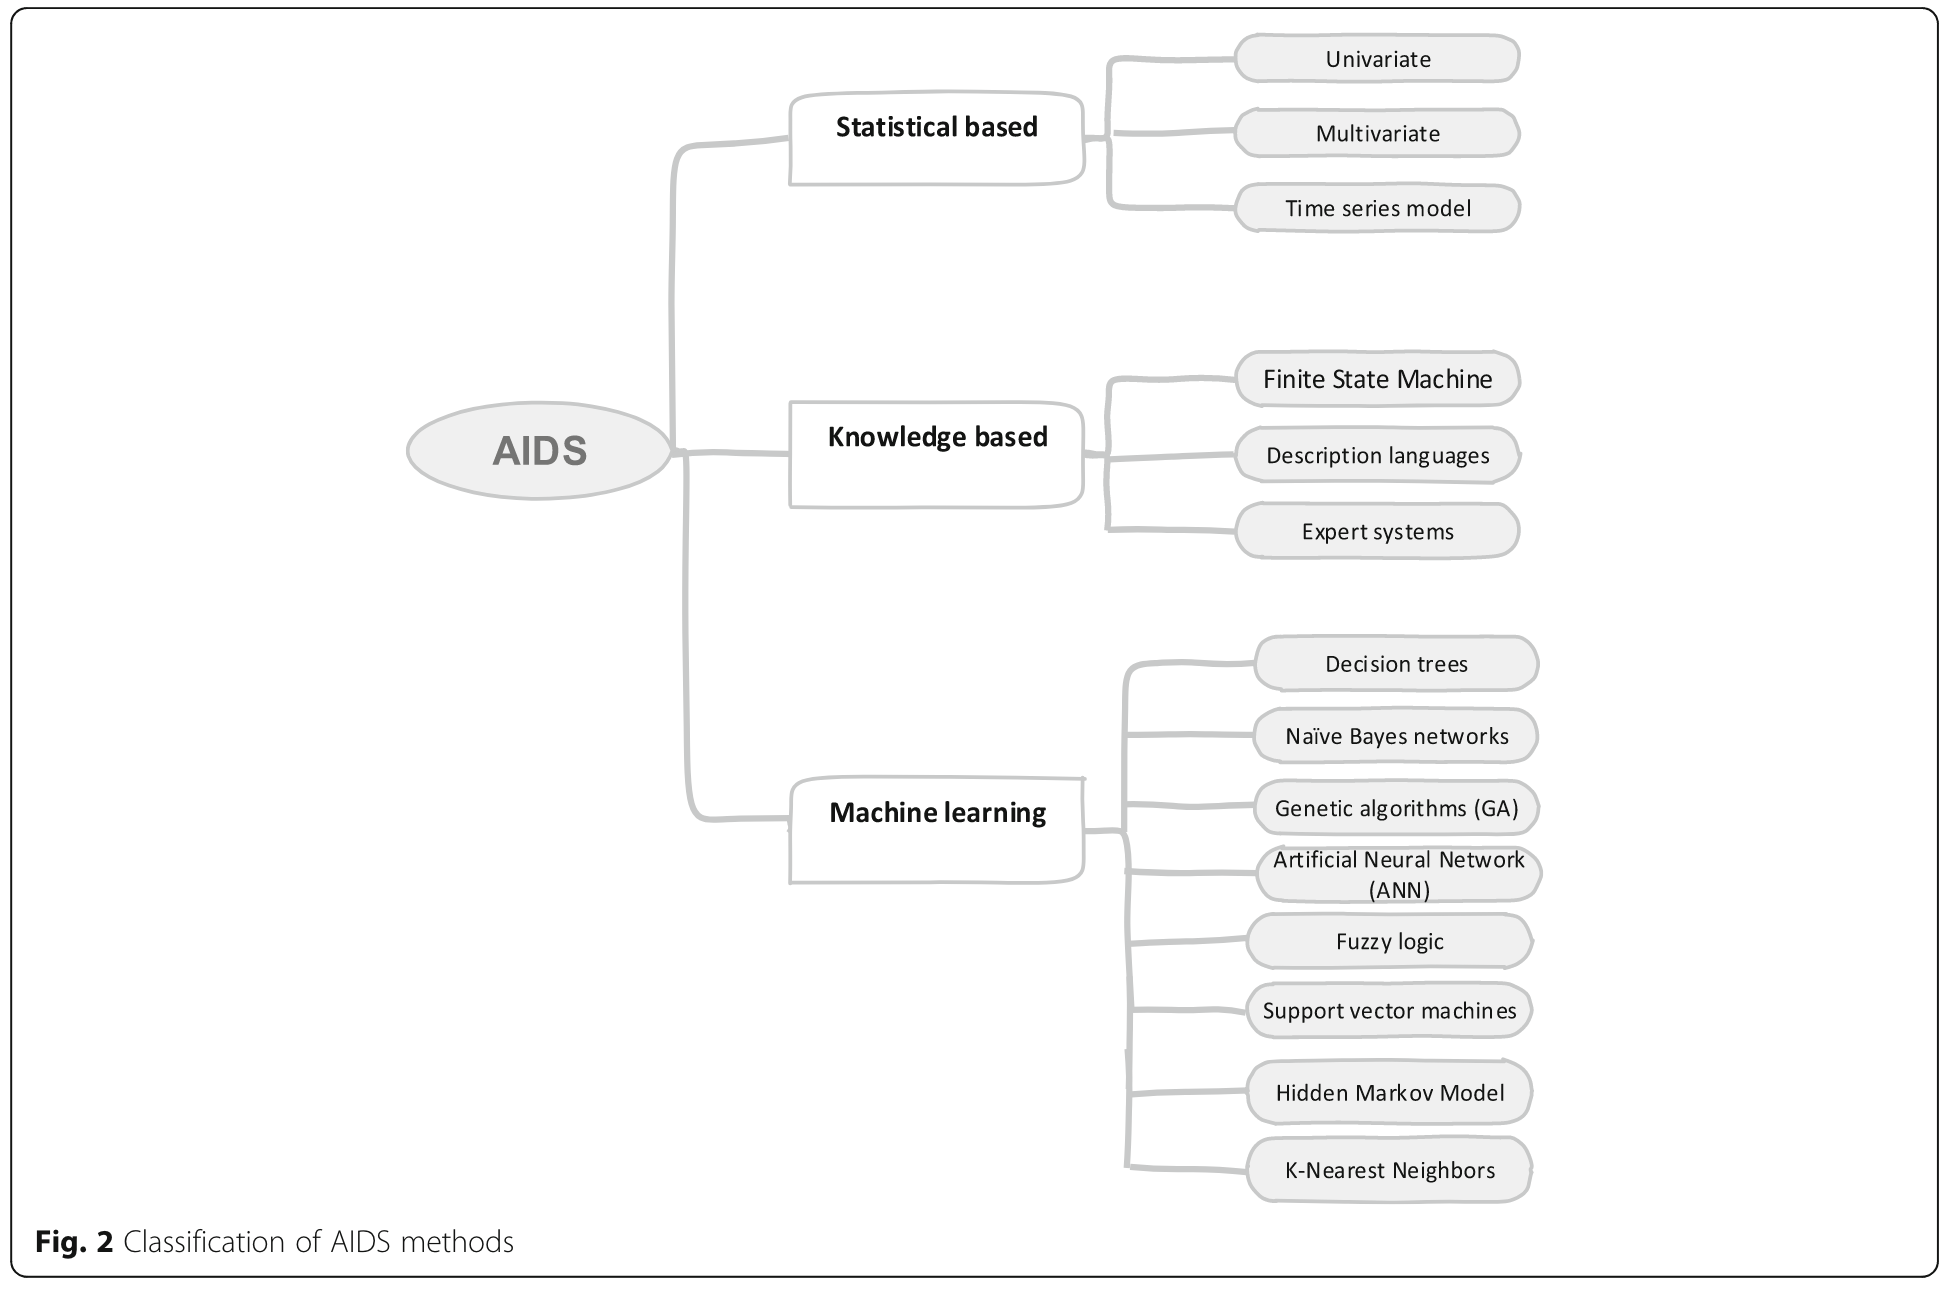
\includegraphics[width=\textwidth,height=10cm,keepaspectratio=true]{img/aids_classification.png}
    \caption{
        Schema che riassume i vari metodi di implementazione degli AIDS, da \cite{SurveyIntrusionDetection2019}. I modelli sono divisi nelle tre categorie descritte precedentemente, ma sono presenti anche i vari tipi di algoritmi utilizzati.
    }
    \label{fig:aids_classification}
\end{figure}


\subsection{Stateful-Protocol-Analysis}

In questo caso gli IDS conoscono lo stato e le specifiche del protocollo utilizzato. Vengono quindi rilevati degli eventi che non rispettano gli standard del protocollo, generalmente quelli da specifica e.g. IEEE.

Potrebbe sembrare che gli AD e gli SPA siano simili, in realtà i primi, conoscono il comportamento di una specifica rete,  mentre i secondi, conoscono solo gli standard dei protocolli.



\section{Machine Learning per rilevamento di intrusioni}


\section{XGboost}


\section{Dataset}


